%----------------------------------------------------------------------
%	CERN TEST BEAM CHAPTER
%----------------------------------------------------------------------
\label{ch:analysis}

Along with determining the focal plane and radiation hardness of the 3-layer lens design, another crucial step towards solidifying an EIC DIRC design was to test the new lens in a prototype DIRC with a real particle beam. Because not all of the components of the high-performance DIRC baseline design for an EIC are currently available it is necessary to validate the simulation package currently used to design and optimize the system. In June and July of 2015 the PANDA Barrel DIRC group along with myself and Dr. Grzegorz Kalicy from CUA conducted a test beam at the European Organization for Nuclear Research (CERN) with a prototype DIRC for the PANDA experiment. This was used as an opportunity to evaluate the performance of the 3-layer lens in a real particle beam. The beam was a hadron-rich beam with momentum tunable from 1 - 10 GeV/c. A standalone GEANT4 simulation package developed for the PANDA DIRC prototype (and later modified for the EIC DIRC geometry) was used for LUT generation, data monitoring, and comparison to data.
%The EIC DIRC simulation package was modified to use this new geometry setup so that data could be compared to simulation. 
The two most important quantities measured during this test beam were the photon yield per track and the single photon resolution (SPR). Verifying these measurements with simulation give a good indication that the performance shown in Chapter \ref{ch:eicdirc} are what should be reasonably expected from a real EIC DIRC detector.

%----------------------------------------------------------------------
%	PROTOTYPE SETUP SECTION
%----------------------------------------------------------------------
\section{2015 Test Beam Prototype Setup}
The PANDA prototype was situated in the CERN Proton Synchrotron (PS) T9 experimental hall \cite{CERN_T9}. A 200 mm thick aluminum target was used to produce a hadron-rich beam comprised mostly of protons, pions, muons, and electrons with a very small amount of kaons. A series of dipole and quadrupole magnets allowed for steering and focusing of the beam, as well as selecting specific particle momenta between 1 and 10 GeV/c for data taking. A scintillator monitored the intensity of the beam and a wire chamber monitored the x/y profile at the exit of the beam pipe.

\begin{figure}[!htb]
	\centering
	\includegraphics[width=\textwidth]{testbeam_2015.pdf}
	\caption{CAD drawing of the T9 experimental hall with the PANDA DIRC prototype setup. Two time-of-flight (TOF) detectors were separated by 29 m and used for proton/pion separation. Two trigger systems were used for the start and stop times of the readout electronics.}
	\label{fig:testbeam_2015}
\end{figure}

A CAD drawing of the experimental setup in the T9 hall can be seen in Figure \ref{fig:testbeam_2015}. The DIRC prototype was situated between two time-of-flight (TOF) detectors that were spaced 29 m apart to tag protons and pions. Figure \ref{fig:TOF_PID} shows the time-based separation of different particle species for 4 different beam momenta. Two scintillator counters (named Trigger 1 and Trigger 2) were placed in front of and behind the prototype. A coincidence of the trigger signals was used as the DAQ event recording trigger. Two veto counters were also set up between the two TOF detectors to reject background particles that strayed significantly from the beam path.

\begin{figure}[!htb]
	\centering
	\includegraphics[width=0.85\textwidth]{TOF_PID.png}
	\caption{Time-of-flight (TOF) particle tagging for 3, 5, 7, and 10 GeV/c beam momentum.}
	\label{fig:TOF_PID}
\end{figure}

\begin{figure}[!htb]
	\centering
	\includegraphics[width=0.6\textwidth]{PANDA_prototype2.pdf}
	\caption{CAD drawing of the 2015 PANDA DIRC prototype setup. The radiator (1), optics (2), expansion volume (3), $3\times5$ array of MCP-PMTs (4), readout (5), and TRB units (6) are supported by an aluminum frame that can move in two directions and rotate, as indicated by the red arrows.}
	\label{fig:PANDA_prototype}
\end{figure}

Figure \ref{fig:PANDA_prototype} shows a CAD drawing of the prototype setup. The prototype was held in place by a custom-built aluminum support structure with rails and a rotating table that allow the detector to be translated and rotated relative to the beam. The rotation of the prototype was verified using a remotely operated motor and camera. The radiator was carefully held in place by two aluminum braces equipped with three micrometer screws which allowed for fine adjustments in the position of the bar. Alignment of all components in the beam line were done with a GLL2-80 Dual Plane Leveling and Alignment Laser by Bosch \cite{BoschLaser}, which provides both vertical and horizontal self-leveled planes. An example of alignment of a radiator plate is shown in Figure \ref{fig:testbeam_alignment}. 

\begin{figure}[!htb]
	\centering
	\includegraphics[width=0.8\textwidth]{testbeam_alignment.JPG}
	\caption{Plate radiator being adjusted by micrometer screws using the Bosch Dual Plane Laser as a guide. When the light reflected off of the radiator lined up with the incoming beam from the laser on the white paper in both the horizontal and vertical directions the radiator was aligned with the beam line.}
	\label{fig:testbeam_alignment}
\end{figure}

\begin{figure}[!htb]
	\centering
	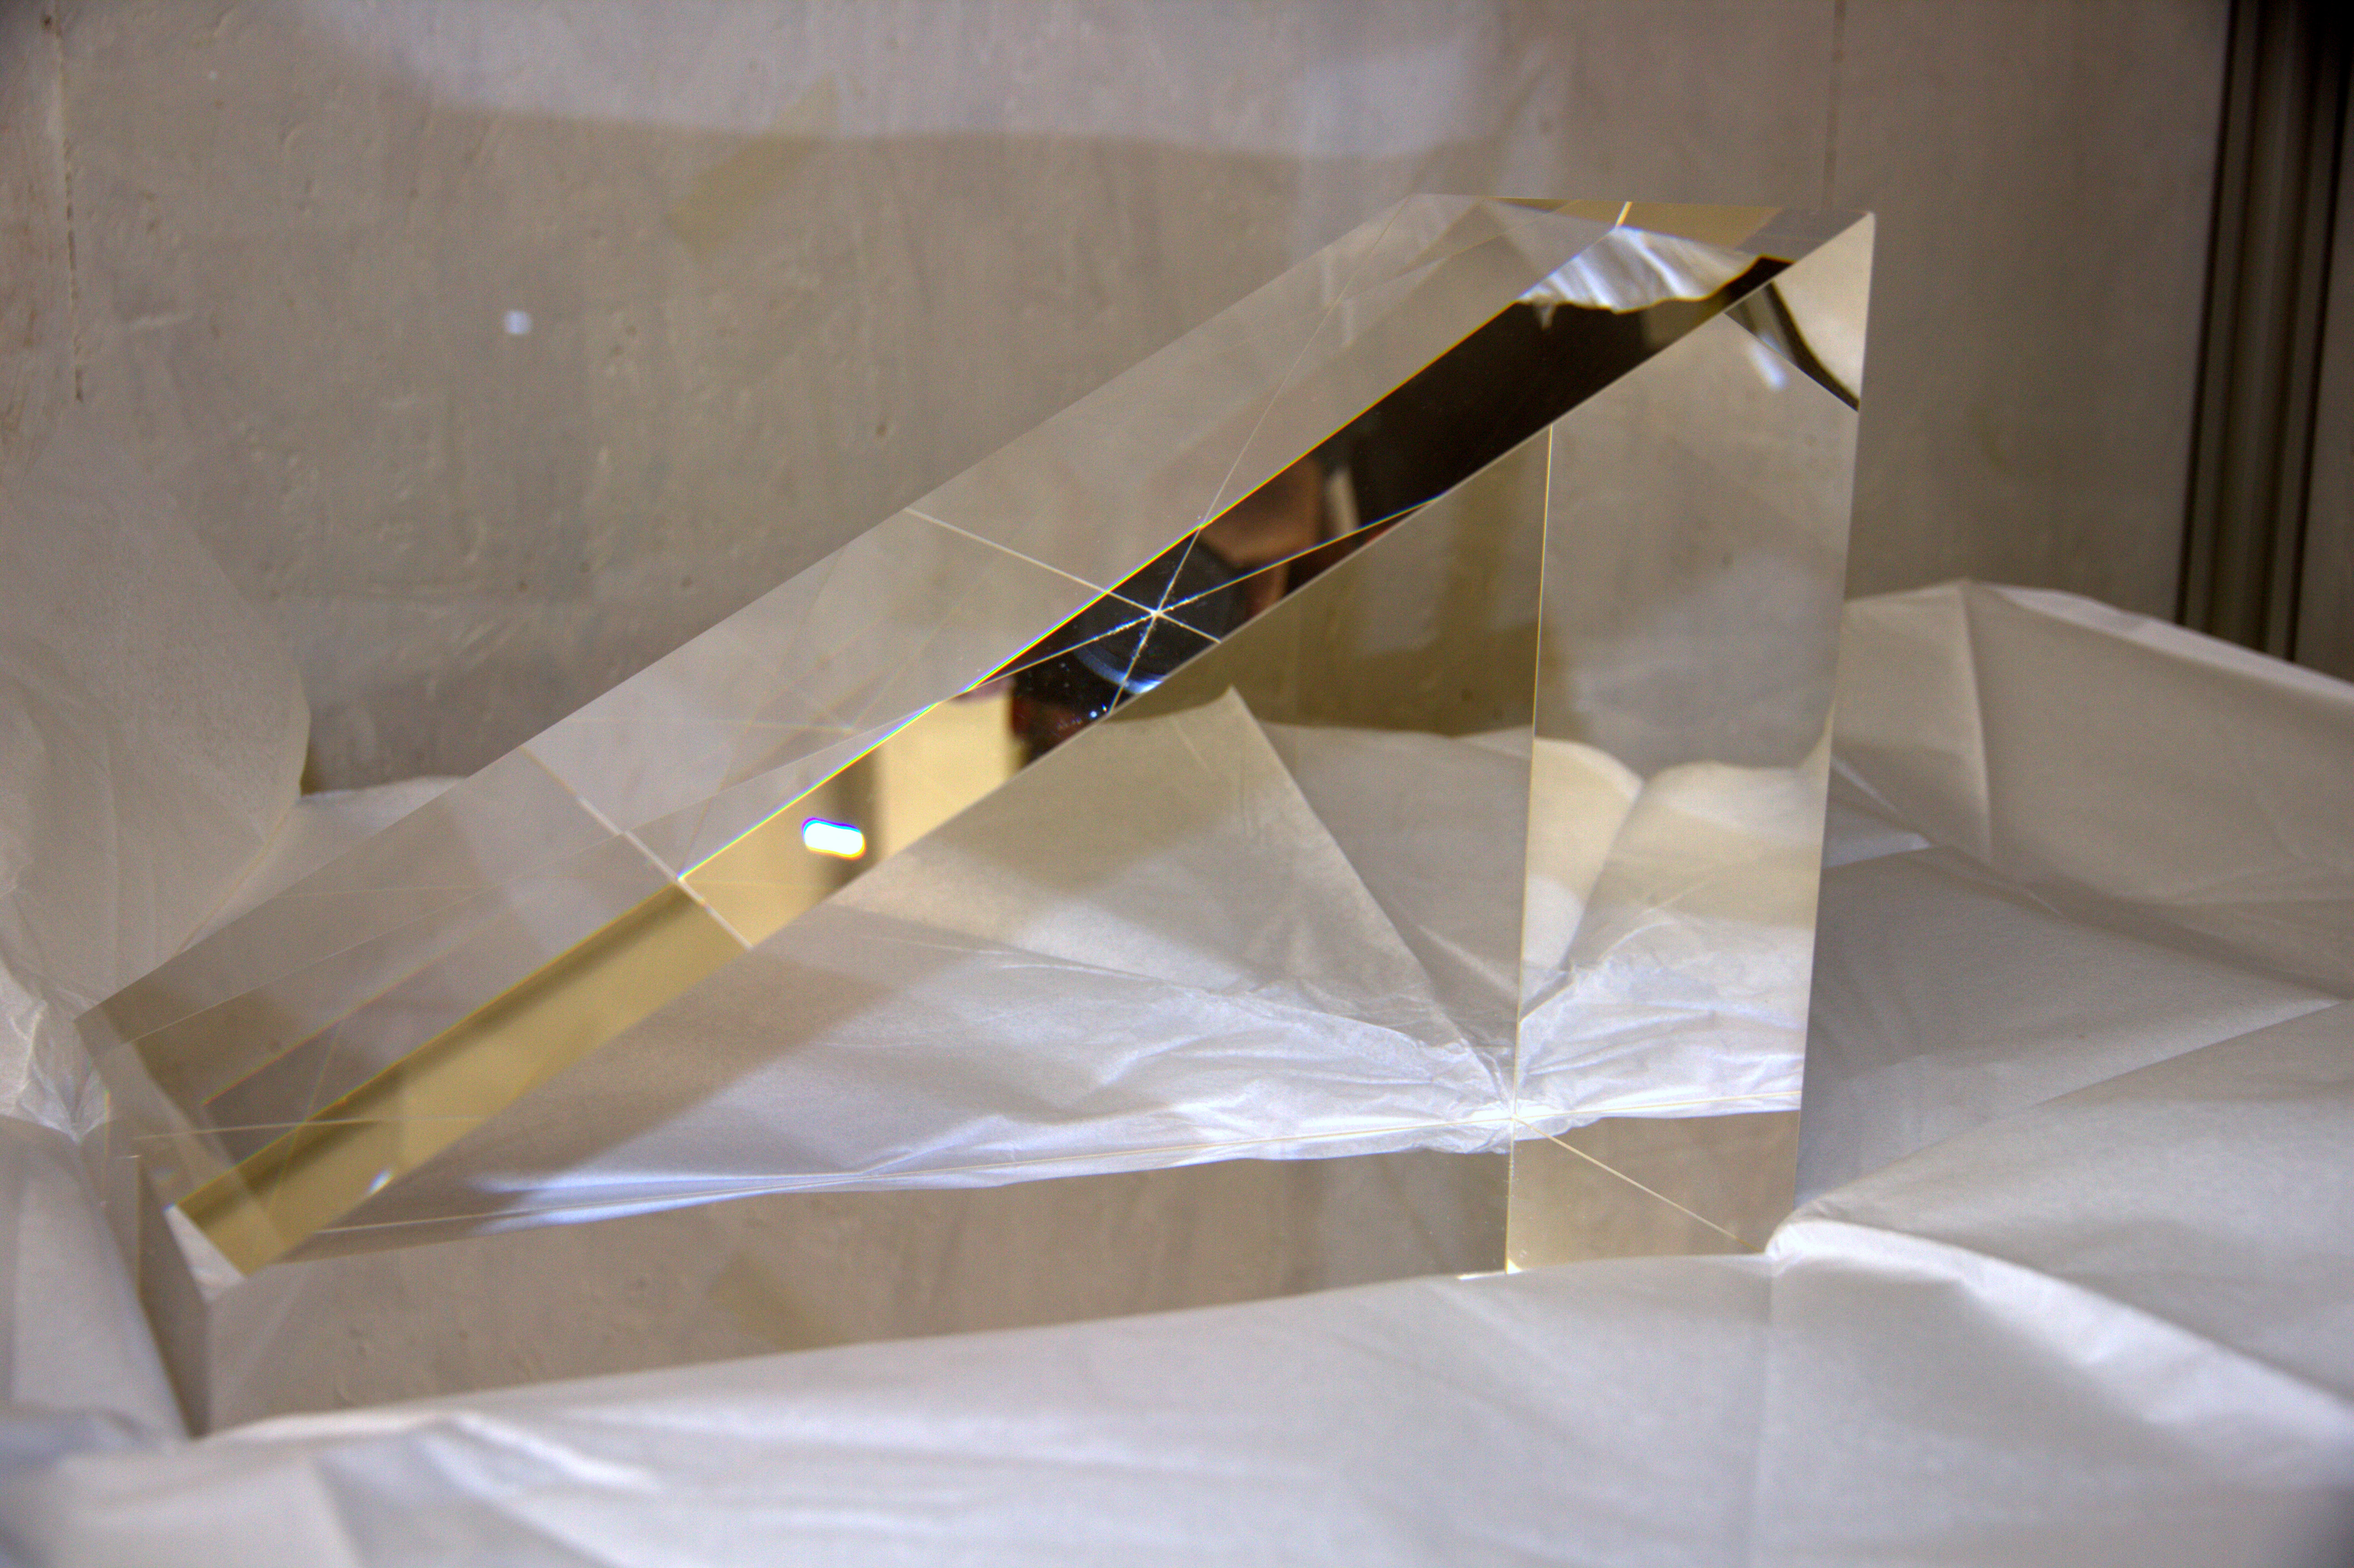
\includegraphics[width=0.7\textwidth]{30-deg-prism.pdf}
	\caption{Picture of the $30^{\circ}$ prism expansion volume used in the 2015 test beam.}
	\label{fig:prototype_prism}
\end{figure}

The optical component is attached to one end of the bar and a mirror is attached to the other. A compact prism expansion volume with dimensions $50\times170\times300\unit{mm}^3$ and an opening angle of $30^\circ$ (shown in Figure \ref{fig:prototype_prism}) was attached to the optical component (except in the case of an air-gap lens). A $3\times5$ array of PHOTONIS Planacon XP85102 MCP-PMTs with a total of 960 pixels were held in place by a support structure and coupled to the expansion volume. The MCP-PMTs were read out by a DAQ system based on the trigger and readout board (TRB3) and the PADIWA discriminator card \cite{PANDA_electronics}. Couplings between the bar/lens, lens/prism, and prism/MCP-PMTs were done using Eljen EJ-550 optical grease \cite{EljenTech}. The mirror was not coupled directly to the bar, but held in place flat against the bar in order to prevent slight variations in grease thickness from effecting the angle of reflection.

The discriminating threshold signals for each MCP-PMT was adjusted and the difference between the discriminator and trigger signals were recorded by the TRB system. Noise events such as photons from delta electrons in the radiator bar and dark noise from the detectors were cut out using this timing information. Some channels had a very large background count rate and were masked. Calibration of the timing resolution of each channel was done using a 405 nm Picosecond Injection Laser (PiLas) PiL040SM by Advanced Laser Diode Systems \cite{PiLas} and a 660 nm Picosecond Pulsed Diode Laser (PDL 800-D) by PicoQuant \cite{PicoQuant}. The laser pulses were connected to an opal glass diffuser to illuminate the entire MCP-PMT plane. Calibrations were performed both daily and any time the geometrical configuration was changed.

Data were taken for approximately 30 days, accumulating roughly 500 million triggers. Both bar and plate radiator geometries were tested with several optical components. Scans in polar angle between $20^\circ$ and $150^\circ$ were taken for many configurations. Scans in momentum up to 10 GeV/c were taken for select angles and geometries. As this was an opportunistic run for the EIC group, data taking was based on the needs of the PANDA DIRC group. They required separation power information for pion/kaon at 3.5 GeV/c, but since the T9 beam had a very small amount of kaons it was decided to instead study pion/proton separation at 7 GeV/c as the difference in Cherenkov angle for both cases is roughly 8 mrad. The results presented below will be from data taken with a bar radiator, 3-layer spherical lens, 7 GeV/c hadron-rich beam, and polar angles from  $20^\circ$ - $150^\circ$.

%----------------------------------------------------------------------
%	SIMULATION SECTION
%----------------------------------------------------------------------
\section{Prototype Simulation}
The simulation of the 2015 prototype was crucial for data analysis as it allowed for the generation of the LUTs for geometrical reconstruction, as well as a reference for the hit patterns \footnote{For the purposes of this document a "hit" or "photon" refers to a signal from a single pixel in an MCP-PMT. However because of an irreducible background it cannot be said for certain which signals are from true Cherenkov photons. What is truely measured are photo-electrons.} of the real-time monitoring system. A standalone GEANT4 simulation package was used, from which the EIC DIRC simulation in Chapter \ref{ch:eicdirc} was produced. Material properties for fused silica, NLaK33, the mirror, the optical grease, and the MCP-PMTs were included. The timing resolution of the simulation was based on findings of the laser calibration data and set to be 200 ps. For each configuration of the prototype the geometry for each element (e.g. relative positioning for the bar to the lens and prism) were adjusted to the values carefully measured while changing configurations.

\begin{figure}[!htb]
	\centering
	\includegraphics[width=\textwidth]{MCP_QE_2015.png}
	\includegraphics[width=\textwidth]{Photonis_QE.png}
	\caption{Channel-by-channel map of the relative quantum efficiency (QE) of each 8x8 pixel MCP-PMT used in the simulation of the 2015 test beam prototype (top). Absolute QE values in the simulation are the product of the channel-by-channel values with the wavelength dependent QE of a Planacon XP85012 MCP-PMT (bottom).}
	\label{fig:quantum_efficiency}
\end{figure}

Also included in the simulation is the quantum efficiency (QE) of the MCP-PMTs. Each MCP-PMT was scanned for QE and gain uniformity with a 372 nm laser pulser at Erlangen University. The mappings of QE were normalized to MCP 10 and used as relative QE maps in the simulation (Figure \ref{fig:quantum_efficiency} top). To get the absolute QE for each pixel a scan was done of the QE as a function of photon wavelength (Figure \ref{fig:quantum_efficiency} bottom). The QE in the simulation was calculated by multiplying the relative QE of each pixel by the QE corresponding to the wavelength of the photon being detected by the pixel in the simulation.

\begin{figure}[!htb]
	\centering
	\includegraphics[width=0.7\textwidth]{proton_track_example.pdf}
	\caption{a) shows a visualization of the GEANT4 simulation of a single 7 GeV/c proton (red) traveling through the 2015 prototype with a bar radiator at a polar angle of $125^{\circ}$, b) is the accumulated hit pattern of 10,000 identical protons from simulation, and c) is the accumulated hit pattern of 10,000 tagged proton tracks from test beam data at 7 GeV/c beam and $125^{\circ}$ polar angle.}
	\label{fig:proton_track_example}
\end{figure}

Figure \ref{fig:proton_track_example}a shows an example of one simulated proton track with 7 GeV/c momentum (red) at a polar angle of $125^{\circ}$ traversing a bar radiator with the 3-layer lens focusing, and producing Cherenkov photons (yellow). Figure \ref{fig:proton_track_example}b is the accumulated hit pattern on the MCP-PMTs of 10,000 identical protons with the same configuration as in (a). Figure \ref{fig:proton_track_example}c is the accumulated hit pattern of 10,000 tagged proton events in the test beam data with 7 GeV/c beam momentum, $125^{\circ}$ polar angle, and the bar radiator and 3-layer lens configuration. The simulation very nicely reproduces the test beam hit pattern, giving a good indication that the simulation has the proper positioning of all the components.

%----------------------------------------------------------------------
%	DATA ANALYSIS SECTION
%----------------------------------------------------------------------
\section{Data Analysis}
\subsection{Event Selection}
The prototype data taken were stored in the list mode data format of the HADES DAQ system prototcol \cite{HADES_DAQ} and converted offline into the CERN ROOT data format \cite{ROOT} for analysis. The DAQ was started by a signal from Trigger 1, and events were required to have signals in Trigger 1, Trigger 2, and both TOF counters to ensure a well-defined beam spot and valid $\pi/p$ tagging from the TOF system. The veto counters were also required in event selection, but later found to be unnecessary for constraining the beam spot.

Hits were selected in a time window of $\pm 40$ ns relative to the Trigger 1 time. Channels with large electronics noise above 1 MHz and one defective PADIWA card were masked, with the same masking scheme applied to the simulation. Events with 5 or fewer MCP-PMT hits were also excluded from reconstruction due to lack of statistics for the reconstruction.

As mentioned previously the timing difference between the two TOF stations allowed for tagging an event as either pion or proton. Figure \ref{fig:tof_timing} shows the TOF time distributions for 5 GeV/c (top) and 7 GeV/c (bottom) beam momenta. These distributions were fitted with Gaussian functions near the proton and pion peaks and a $\pm2\sigma$ window around the peaks was used for selection (dashed lines).

\begin{figure}[!htb]
	\centering
	\includegraphics[width=\textwidth]{TOF_timing.pdf}
	\caption{Time difference between the two TOF stations for beam momenta of 5 GeV/c (top) and 7 GeV/c (bottom). The peaks were fitted and a $\pm2\sigma$ selection window was taken (dashed lines).}
	\label{fig:tof_timing}
\end{figure}

The timing of the hits in the MCP-PMTs were also constrained. Based on the orientation of the detector in the beam the time for the photon to propagate can be calculated, giving an expected arrival time. Comparing the difference between this expected arrival time and the actual arrival time of the photons gives a time difference distribution, shown in Figure \ref{fig:time_difference}. In simulation it is to possible exclude times associated with incorrect reconstructed paths from the LUT. Using this time distribution from only correct simulated paths it was determined that a time difference cut of $\pm1$~ns was sufficient for geometric reconstruction.

\begin{figure}[!htb]
	\centering
	\includegraphics[width=\textwidth]{time_difference.png}
	\caption{Time difference distribution experimental data (black), full simulation (red), and simulation including only correct prism paths from the LUT (blue) for $125^\circ$ polar angle. The dashed lines indicate the $\pm$1~ns cut taken for during analysis.}
	\label{fig:time_difference}
\end{figure}


\subsection{Geometrical Reconstruction}

\subsubsection{Charge Sharing Correction}
It was discovered that many events in the prototype data showed multiple adjacent MCP-PMT pixels firing in a single event. It is difficult to say with certainty if neighboring firing pixels, such as the example shown in Figure \ref{fig:charge_sharing}a, fired independently or if charge sharing between the pixels occurred, effectively spreading the pixel's signal across multiple pixels. Because the width of each pixel corresponds to roughly a 20~mrad spread in Cherenkov angle the results of reconstructing these clustered pixels with the standard averaged LUT resulted in wider than expected reconstructed Cherenkov angle distributions for the prototype data. 

The solution was to modify the LUT to reconstruct the position of the photon not from the center of each pixel, but towards an edge, weighted by the position of neighboring firing pixels. Each pixel is subdivided into 9 sections in the LUT, as in Figure \ref{fig:charge_sharing}b. The reconstruction algorithm first determines if and where adjacent firing pixels are located for each hit and then reconstructs the Cherenkov angle at the center of the section most heavily weighted. Figure \ref{fig:charge_sharing_reco} shows the effect of this charge sharing correction for simulation (top) and experimental data (bottom) at $90^\circ$ polar angle. As was expected, the simulation, which does not include charge sharing, was largely unaffected. In the prototype data, however, the correction served to narrow the reconstructed Cherenkov angle peak and reduce background contributions.

\begin{figure}[!htb]
	\centering
	\includegraphics[width=\textwidth]{charge_sharing.pdf}
	\caption{a) a zoom in on a single MCP showing an example hit pattern from a single particle track. The 3 isolated pixels (red) have no neighboring hits. The 3 clustered hits (green), however, are adjacent to other firing pixels and thus it is hard to determine with timing alone if these are the result of a single photon from the bottom right pixel that resulted in charge sharing, 3 independent photons hitting all 3 pixels, or some combination of 2 photons hitting 2 of the pixels that resulted in charge sharing. To compensate for this uncertainty each pixel is subdivided, as in (b), into 9 regions such that the LUT will reconstruct the photon angle from different areas of the pixel. For the case of (a) the top pixel in the cluster would be reconstructed from point 7, the bottom left pixel from point 5, and the bottom right pixel from point 2, while the 3 isolated pixels would all be reconstructed from point 0.}
	\label{fig:charge_sharing}
\end{figure}

\begin{figure}[!htb]
	\centering
	\includegraphics[width=\textwidth]{chargeshare_90_sim.png}
	\includegraphics[width=\textwidth]{chargeshare_90_data.png}
	\caption{Reconstructed Cherenkov angle of 7 GeV/c protons for simulation (top) and prototype data (bottom) for $90^\circ$ polar angle using the standard LUT (blue) and the charge-sharing-corrected LUT (red). The simulation is largely unaffected, while in the data the peak has been narrowed and the background reduced.}
	\label{fig:charge_sharing_reco}
\end{figure}


\subsubsection{Per-MCP-PMT $\theta_{C}$ Correction}
The fitted mean of the reconstructed Cherenkov angle from geometric reconstruction showed a non-constant value across the prototype polar angle range for both simulation and experimental data. To correct for this non-constant shift a per-MCP-PMT $\thetaC$ correction was implemented in the reconstruction. For a given polar angle and particle species the reconstructed Cherenkov angle for each MCP-PMT is fitted in the same manner as the full data set and a value for the Cherenkov angle is extracted (see Figure \ref{fig:mcp_corr_hist}). The difference between the extracted value and the true value define a shift that is then used to adjust the Cherenkov angle spectrum for each individual MCP-PMT. After corrections the mean Cherenkov angle is much more accurately reproduced, and even improves the SPR at the some polar angles. Figure \ref{fig:mcp_corr_polar} shows the results of the correction for the full range of polar angles.

\begin{figure}[!htb]
	\centering
	\includegraphics[width=\textwidth]{mcp_corr_hist.png}
	\caption{Reconstructed $\thetaC$ at $90^\circ$ polar angle before (red) and after (blue) per-MCP-PMT corrections. The uncorrected distribution has a mean $\thetaC$ of 823.1 mrad, or 6.3 mrad away from the true value of 816.8 mrad for a 7 GeV/c proton. The corrected distribution has a mean of 813.4 mrad, which is only 3.4 mrad away from the true value.}
	\label{fig:mcp_corr_hist}
\end{figure}


\begin{figure}[!htb]
	\centering
	\includegraphics[width=\textwidth]{mcp_corr_polar.pdf}
	\caption{\textbf{Top}: Reconstructed mean $\thetaC$ before applying per-MCP-PMT corrections for simulation (blue) and prototype data (red) for 7 GeV/c protons. The dashed line indicates the true Cherenkov angle for a 7 GeV/c proton. \textbf{Bottom}: Reconstructed $\thetaC$ after applying corrections.}
	\label{fig:mcp_corr_polar}
\end{figure}


\subsubsection{Simulated Background Subtraction}
Because the majority of the background signal for the reconstructed Cherenkov angle comes from irreducible ambiguities it would stand to reason that the ambiguity background simulated in GEANT4 would reasonably describe the PANDA prototype background seen in the experimental data. Figure \ref{fig:background_sub}a shows a simulation of 1000 protons at 7 GeV/c and $125^\circ$ polar angle along with the ambiguity background (i.e. the reconstructed Cherenkov angle coming from incorrect prism ambiguities) and the reconstructed angles coming from true prism paths. Figure \ref{fig:background_sub}a shows the prototype data with the same configuration along with the simulated background and the background-subtracted data. Because of the nice description of the background from simulation, the background-subtracted prototype data shows a clear peak and minimal background. This method 

\begin{figure}[!htb]
	\centering
	\includegraphics[width=\textwidth]{background_subtraction.pdf}
	\caption{The full reconstructed Cherenkov angle (blue line), incorrect prism path ambiguities (black circles), and the reconstructed Cherenkov angle assuming only true prism paths (red area) for $125^\circ$ polar angle protons from simulation (a) and beam data (b).}
	\label{fig:background_sub}
\end{figure}

\subsubsection{Error Evaluation (Evaluation of Uncertainties?)}
file internal consistency (e.g. comparing every 100 events)

varying gaus+background fit and range

reproducibility from different runs (comparing 151 to 158)

varying timing cut

varying binning size

\subsubsection{Results}

\subsection{Time-based Reconstruction}

\subsubsection{Results}
